\label{intro-chapter}
\section{Challenges in Security Reasoning}
\label{intro-challenges}

Information-flow security is highly desirable in today's real-world software.
Hackers often exploit software bugs to obtain information about 
protected secrets, such as user passwords or private keys. 
Security issues have become even more of a concern in recent
times with the advent of cloud computing and distributed 
architecture, since many mutually-distrusting users 
execute over the same physical hardware.

It is extremely difficult to justify that a piece of software
protects users' secrets. Virtually any bug could lead to
an exploitable security hole, and reasoning about security
is still difficult even when software is known to be 
functionally correct. It is therefore logical to look to formal 
methods for providing a foundation for complex security reasoning.
There have been many diverse attempts in the literature, especially 
over the last two decades, at formally guaranteeing software security.
These attempts include techniques like adding dynamic security 
monitors to runtime environments (e.g.,~\cite{austin09,guernic07,venkat06,shroff07}), 
statically bounding software 
with security-aware type systems or logics (e.g.,~\cite{jif,slam,hunt06,banerjee08}), 
and reasoning about the
implications of various kinds of high-level security policies
(e.g.,~\cite{rhtt,sabelfeld99}).
The state-of-the-art is not entirely satisfactory, however,
as each of these individual security-reasoning methodologies is 
relatively limited in scope. Our ultimate goal in this dissertation 
is to demonstrate the possibility of a highly general methodology,
that allows for both formally specifying any desired information-flow 
security policy, as well as formally guaranteeing that the low-level code 
of a complex system conforms to this high-level policy.

\begin{comment}
Information flow control (IFC)~\cite{myers-liskov,sabelfeld03} is a
form of analysis that tracks how information
propagates through a system. It can be used to state and verify
important security-related properties about the system.  In this work,
we will focus on the read-protection property known as
\emph{confidentiality} or \emph{privacy}, using these terms
interchangeably with security.
\end{comment}

%%%%%%%%%%%%%%%%%%%%%%%%%%%%%%%%%%%%%%%%%%%%%%%%%%%%%%%%%%%%%%%%
\begin{figure}[t]
\begin{center}
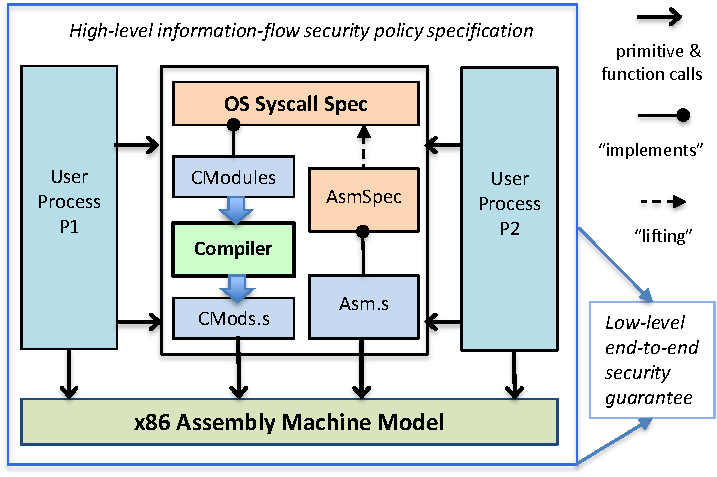
\includegraphics[scale=0.685]{pldi/figure/osmach2}
\caption{\small An end-to-end software system that consists 
of both OS modules (in C and assembly) and user processes.}
\label{fig:osmach}
%\vspace*{-20pt}
\end{center}
\end{figure}
%%%%%%%%%%%%%%%%%%%%%%%%%%%%%%%%%%%%%%%%%%%%%%%%%%%%%%%%%%%%%%%%

There are all kinds of challenges that we must overcome to achieve 
such a lofty goal. Consider the example setup of 
Figure~\ref{fig:osmach}, where a large operating system kernel
consists of many separate functions (e.g., system call primitives) 
written in either C or assembly. Each primitive has a
high-level specification, and there is a compiler that converts
all C code into assembly. User processes execute arbitrary 
assembly code over the kernel, and they may occasionally 
invoke the kernel system calls. In order to achieve our desired 
goal, we must be able to clearly and formally specify a high-level
security policy over this entire system, and we must be able to
provide an \emph{end-to-end} guarantee that all of the code,
when linked together and executed over the x86 machine model,
conforms to the security policy. We now describe the major
challenges involved, contextualized with the help of this example.

\paragraph{Challenge 1: Policy Specification}
How do we specify a clear
and precise security policy, describing how information is
allowed to flow between various users? If we express the
policy in terms of the high-level syscall specifications, 
then what will this imply for the whole-program assembly execution? 
We need some way of interpreting and enforcing policies at different 
levels of abstraction. Furthermore, it is crucial that the
high-level policy language is expressive enough to handle more
than just pure isolation. In the real world, users often wish to
communicate with each other in certain ways; thus we must support
policies which allow certain well-specified forms of 
communication, including controlled declassifications of 
data from a high security level to a lower one.

\paragraph{Challenge 2: Reasoning About Low-Level Code}
Assuming we can specify a security policy at a low level of
abstraction, how should we go about proving that some low-level
C or assembly code conforms to the policy? Security-aware type
systems like Jif~\cite{jif} do not work well for untyped
languages, while dynamic security monitors incur undesirable execution 
overhead. Incompleteness is also problematic: a low-level program
may execute an action that temporarily violates a security policy, 
but then the program does not end up producing any observable
behaviors influenced by the violation. For example, for performance
reasons, a program might read an entire block of a file into memory,
despite not actually needing to know any secret 
data stored within that block. The end-to-end behavior of such a 
program is secure, but many line-by-line security enforcement
mechanisms will deem it insecure.

%It is well known~\cite{jurjens,morgan09} that
%simulations and refinements may not propagate security guarantees.
%How, then, can we soundly obtain a low-level guarantee from a 
%high-level security verification?

\paragraph{Challenge 3: Linking Everything Together}
Multiple aspects of Figure~\ref{fig:osmach} require linking:
C code must be linked with assembly code within the kernel, 
low-level C and assembly code must be linked with their 
high-level specifications, and user code must be linked
with kernel code. Even if we manage to prove security of
each of the individual pieces (kernel C functions, kernel
assembly functions, arbitrary user code, and high-level
specifications), how are we going to guarantee end-to-end
security when all of these pieces are combined together?
Simulations or refinements are generally used to link low-level
code with high-level specifications, but it is well 
known~\cite{jurjens,morgan09} that these may not soundly propagate 
security properties like noninterference. Furthermore, linking C 
code with assembly code requires compilation; modern C compilers usually 
have bugs causing program functionality to not be correctly preserved, 
and they certainly do not make any attempts to preserve security.

\section{Contributions}
In this dissertation, we successfully achieve our goal by
showing how all of the challenges mentioned above can be cleanly
handled. We make two major contributions: we design a novel
methodology that achieves our goal, and we apply the methodology
to guarantee security of an actual system.

%%%%%%%%%%%%%%%%%%%%%%%%%%%%%%%%%%%%%%%%%%%%%%%%%%%%%%%%%%%%%%%%
\begin{figure}[t]
\begin{center}
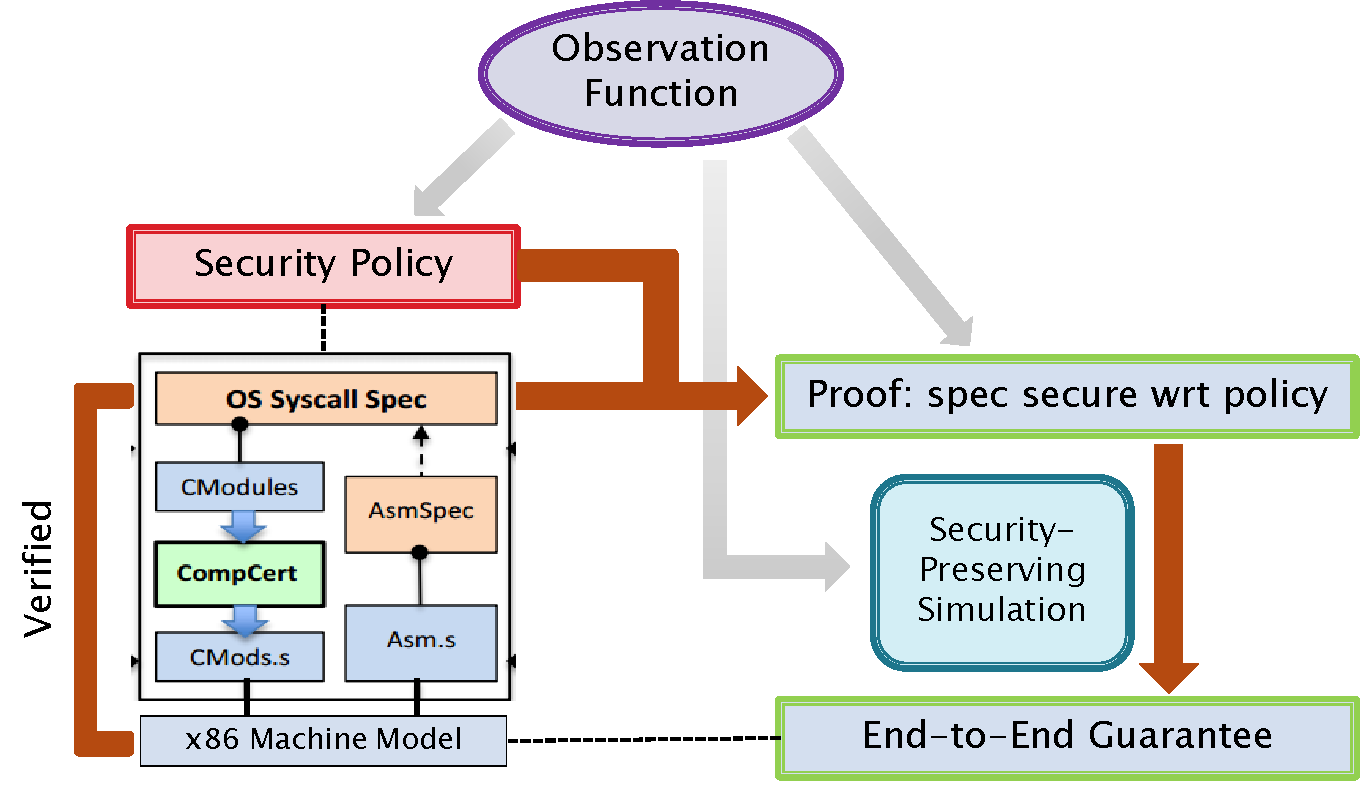
\includegraphics[scale=0.5]{pldi/figure/methodology}
\caption{\small Using an observation function to verify end-to-end
security.}
\label{fig:methodology}
%\vspace*{-20pt}
\end{center}
\end{figure}
%%%%%%%%%%%%%%%%%%%%%%%%%%%%%%%%%%%%%%%%%%%%%%%%%%%%%%%%%%%%%%%%

\paragraph{Contribution 1: Novel Methodology}
The first contribution is the development of a novel and
highly-general methodology allowing us to formally specify, verify, 
and link security policies. Figure~\ref{fig:methodology}
gives a broad overview of our design. We first require that
functional correctness is verified independently from security: 
all of the code must be shown to conform to the high-level 
specifications. Then, for the security verification, we
begin by defining an ``observation function'', which essentially 
describes each user's view of program state. This observation
function automatically induces a high-level security policy.
Next, the system's high-level specification is verified to conform
to the induced security policy. Finally, this high-level security 
property is automatically propagated down to a low-level, end-to-end
guarantee by exploiting a special kind of simulation that soundly
preserves security.

\paragraph{Contribution 2: Applying the Methodology}
We demonstrate the effectiveness of this novel methodology by
applying it to real operating system kernel,
called mCertiKOS. As described in~\cite{certikos-popl}, 
mCertiKOS is already fully verified to be functionally correct
with respect to high-level specifications; thus our security
verification effort does not require the first step described in 
Figure~\ref{fig:methodology}. Our resulting artifact,
called mCertiKOS-secure, is the first
ever guaranteed-secure kernel involving both C and assembly code,
including compilation from the C code into assembly (which is handled
by the CompCert verified compiler~\cite{compcert}). Our final
result guarantees the following notion of isolation: as long as 
direct inter-process communication is not used, user processes 
executing over the kernel cannot influence each others' executions 
in any way. During the verification effort, we successfully 
discovered and fixed some interesting security holes in the kernel, 
such as one that exploits child process IDs as a side channel. 
After completing the verification, we tested the
extensibility of our methodology by adding a new feature to the
kernel providing users with a notion of time. With relatively
little effort we were able to prove security of the new feature,
guaranteeing the absence of any timing-based information-flow side 
channel.

\paragraph{Previous Efforts}
While the most important contributions in this dissertation are
the two just described, we spent multiple years trying other
strategies before arriving at our
new methodology. We will devote two chapters to describing 
these earlier efforts, as they illustrate numerous important
concepts that are used as stepping stones toward developing our
ultimate contribution. The first of these chapters describes our work
published in APLAS~\cite{costanzo-bpsl}, in which we argue that 
systems should enforce a strong notion of locality, guaranteeing
that unused resources never affect program behaviors. While
we did not have security in mind at the time, it turns out that
this strong locality has close ties with composability of
secure systems. The second chapter describes our work published
in POST~\cite{costanzo-ddifc}, in which we present a new program logic
that allows one to specify and prove very general security 
policies over C-like code. The program logic only applies to
code written in the C-like language, so it only solves a 
small portion of the challenges described in 
Section~\ref{intro-challenges}.

\paragraph{Machine-Checked Verification}
All of the work throughout this dissertation is fully
formalized and verified in the Coq proof assistant~\cite{coq}.
This means that all proofs are machine-checked, and therefore bug-free.
The Coq formalizations, including the entirety of the secure
mCertiKOS kernel, can be found online at this dissertation's
companion website~\cite{costanzo-thesis}.



\ignore{
The following concepts can be formulated in terms of 
observation functions:
\begin{itemize}
\item \emph{Policy}~--- Given a principal $l$ and program state 
$\sigma$, an observation function induces a security policy
stating that there is no flow of information to $l$ from 
anything in $\sigma$ outside of 
$l$'s observation. In fact, we do not technically require 
observations to be a portion of program state; they can be any
arbitrary transformation on state. This allows us to express a
variety of security policies with % , including some kinds of 
declassification~\cite{sabelfeld-sands}. 
% We will present some examples of interesting 
% policies in Section~\ref{informal}.
\item \emph{Indistinguishability}~--- Two program states are
considered to be indistinguishable to $l$ just when $l$'s observations
on the states are identical.
\item \emph{Whole-Execution Observations}~--- Certain ``well-behaved''
types of observations, such as an append-only output buffer, can be 
used to describe global execution observations, or \emph{behaviors}. 
For example, an execution may have the behavior
``termination with final observation $o$''. We express security of 
the low-level system implementation in terms 
of whole-execution behavioral equality, since the high-level 
unwinding condition does not propagate across simulation.
\item \emph{Linking}~--- We use different observation
functions for different levels of abstraction. This means that we
can use an observation function mentioning machine registers to 
verify an assembly primitive, and a different observation function
mentioning program variables to verify a C primitive. These
observation functions are linked across abstraction levels via
a special kind of simulation that preserves state
indistinguishability.
\end{itemize}
}
%%%%
\begin{comment}
Note that none of these three aspects is individually novel. The
described security proof is a standard method for proving noninterference, 
known as \emph{unwinding}~\cite{goguen82,goguen84}.
The idea of preserving security across simulation or refinement has been 
explored in previous literature, such as~\cite{jurjens,morgan09,murray12}.
Expressing security policies in terms of an abstract notion of
observation or observable equivalence has also been 
explored~\cite{costanzo14,rhtt,sabelfeld99}. Our main contribution
in this work is to unify all three of these aspects with the \emph{single} 
concept of a general observation function. 
\end{comment}
%%%%

\begin{comment}
\cut{
Note that, while most of the mCertiKOS code is written in C and compiled into
assembly by CompCert, there are some primitives that must be written directly
in assembly. Context switch is a classic example of such a primitive.
The primary functionality of a context switch 
involves copying values between machine registers and kernel objects;
hence both the implementation and specification of the primitive 
must refer to low-level machine state. A key goal and contribution of
our security verification is that assembly primitives like context
switching are fully handled within the framework, and thus do not need to
be trusted.}
\end{comment}

\section{Principals and Policies}
\label{intro-policies}

In this section, we informally introduce some basic terminology that 
will be heavily used throughout the dissertation. We also describe
some motivating example security policies that will occasionally
be revisited in later chapters.

Assume we have a complex system like the one from
Figure~\ref{fig:osmach}, which is composed of many lines of both C and assembly code.
As described previously, we wish to prove the end-to-end property that, when the 
C code is compiled into assembly and linked with the existing assembly code, the resulting 
system executes securely. More specifically, we will prove that a system executes
securely with respect to a particular \emph{principal's} point-of-view; this particular
principal is called the \emph{observer}. Principals
represent actors or users of the system (e.g., processes $P1$ and $P2$ are principals
of the system in Figure~\ref{fig:osmach}), and we will assume they come from some
abstract set $\princ{}$.

For each potential observer $p$, we will specify a \emph{security policy} describing 
precisely how information can flow to $p$. A system is then deemed secure if and only if 
it obeys all observers' policies. As described in Section~\ref{intro-challenges}
above, exact formalization of a security policy 
represents a major challenge in any information-flow system. To support real-world
systems, it is crucial that policies allow for certain well-specified flows of 
information (e.g., declassifications); however, it is in general not obvious how
to define an end-to-end security guarantee with respect to such lenient policies.
To develop some intuition regarding this challenge, we will now consider some
example security policies that are important to support.

\paragraph{Public Parity}
Suppose principal Alice owns some secret value $v$. Alice wishes to release
only a single bit of her secret publicly, the parity $v\%2$. Describing this
as a somewhat more formal security policy, we say that the observations made by 
any observer $p$ (excluding Alice) must not be influenced by anything relating 
to $v$ other than its parity. This statement can be clearly expressed 
as a noninterference-like property: if we were to hypothetically
change Alice's secret from $v$ to any other value $w$ with the same parity 
as $v$, then observer $p$ must make identical observations over the system 
executing with secret $w$ as it does over the execution with secret $v$.

Notice that
there is some implicit subtlety in the described policy: if an observer can 
learn the value $v\%2$, then clearly he can also learn, for example, the value 
$(v+1)\%2$. This implicitly-derived kind of information flow can become difficult
to understand for extremely complex policies; we will assume throughout the
dissertation that it is the system specifier's burden to write a policy that
is simple enough for users of the system to fully comprehend.

\paragraph{Public Average}
Suppose Alice runs a company and stores all employees' salaries in a database.
One reasonable security policy is to publicly release only the average of these 
salaries. That is, there should be no flow of information from the salaries to 
public observers other than the value of the average salary. As a noninterference statement,
this means that if we were to change the values of any subset of salaries in
such a way that the overall average remains the same, then a public observer
must not see any change in observation. Furthermore, one might reasonably
extend the policy to apply to an employee $p$ of the company by allowing $p$
to learn information only about $p$'s own salary, in addition to the average
salary. Note that, once again, there is some implicit information embedded
in this policy: if, for example, $p$ happens to know that there are only two employees in
total at the company, then he can learn the exact value of the other employee's
salary just by looking at his own salary along with the average. Thus this
policy would only be a reasonable one for security purposes if there were many 
employees at the company.

\paragraph{Shared Calendar}
As a more intricate example, suppose Alice owns a calendar on which she
marks down the details of various events occurring at various time slots.
Further suppose that Alice wishes to expose an API for her calendar that
allows other principals to schedule a meeting with her at an open time slot.
What kind of security policy might Alice wish to enforce over her calendar?
An initial guess might be that Alice should not release any information
about her calendar; this is incompatible with the desired API, however, since
a principal who successfully schedules a meeting with Alice will obviously
learn that the scheduled time was available in her calendar. Instead, a
more reasonable policy is that a caller of Alice's API can learn which time
slots are available/unavailable in the calendar, but cannot learn any 
information about the events contained within the unavailable slots.

In terms of noninterference, this policy says that if we were to arbitrarily
change the events within Alice's calendar without changing any times at
which those events occur, then a caller of Alice's API would not observe any
difference. One example implementation that clearly satisfies this security
policy is for Alice to always schedule the meeting at the first available 
time slot.

\paragraph{Dynamic Label Tainting}
One common and important example involves attaching security labels to 
principals and data within a system, and then dynamically propagating 
(``tainting'') these labels 
as the system executes. Many existing security frameworks are based upon
this scheme (e.g.,~\cite{austin09,zdancewic02,hritcu13,flume,resin}). Security labels are arranged into
a lattice structure where, for example, $L_1 \sqsubseteq L_2$ means that the
security level $L_2$ is ``at least as secure as'' level $L_1$. An element of
this lattice is assigned to each principal and each piece of data
within the system. The standard security policy is then that information is 
only allowed to flow up this lattice~--- that is, an observer $p$ with
label $L_p$ can only learn information about data with label less than or
equal to $L_p$ in the lattice. As a noninterference statement, this means 
that changing any data with a label $L \not\sqsubseteq L_p$ will
not affect $p$'s observation.

A simple method for enforcing this security policy is to dynamically 
taint data as it propagates during an execution. For example,
if the program $z = x + y$ executes, then the resulting security label 
of $z$ will be assigned the least upper bound ($\sqcup$) of the labels 
of $x$ and $y$. In this way, the system can automatically guarantee that
the resulting value of $z$ can flow to some principal $p$ (i.e., 
$L_x \sqcup L_y \sqsubseteq L_p$) if and only if the values of $x$ and $y$ 
can also flow to $p$ (i.e., $L_x \sqsubseteq L_p$ and $L_y \sqsubseteq L_p$).

\paragraph{Aside on Declassification Terminology}
Traditionally, declassification is a term used in a context like the 
dynamic label tainting just described, where the security label of a 
piece of data is explicitly changed from some $L$ to some $L'$ with
$L \not\sqsubseteq L'$. Declassifications may violate the policy that information
can only flow up the lattice, and therefore many systems must carefully 
specify precise conditions under which declassifications are allowed to occur. 
Throughout this dissertation, we will refer to this concept as
an ``explicit declassification''. One thesis of our work is that it
is generally difficult to express a formal end-to-end security property
for a system that allows such explicit declassifications. In this work,
we instead support what we call ``implicit declassifications''~---
a concept which we will show yields a clean and descriptive end-to-end security 
property. For example, in the public parity example described above, we say that Alice
is ``implicitly declassifying'' the value $v\%2$ from secret to public. That
example is not an explicit declassification because there are no explicit
labels attached to the data.

In general, it is not possible to give any kind of formal 
definition to our notion of implicit declassification. As described above,
an implicit declassification of $v\%2$ automatically implies implicit declassification
of $(v+1)\%2$. Furthermore, we will see an example later in the dissertation,
relating to the mCertiKOS security verification, where a policy seems to
describe an implicit declassification, but actually does not allow information
to flow from high security to lower security. In other words, there is no clear relationship
between implicit declassifications and the allowed information flows. As a result,
all uses of the term ``declassification'' in this dissertation should be interpreted in 
an informal context; our security policies will formally and precisely specify how 
information is allowed to flow between principals, but they will not formally specify 
whether or not declassifications are allowed.

\section{Chapter Organization}
The rest of this dissertation is organized as follows. 
Chapter~\ref{bpsl-chapter} is an abridged version of our work
published in~\cite{costanzo-bpsl}, and discusses strong locality.
There are some interesting connections between locality and security, 
but overall the chapter is fairly orthogonal to the rest of the dissertation. 
Chapter~\ref{logic-chapter} is an abridged version of our work
from~\cite{costanzo-ddifc}, and attempts to tackle security verification
by using a program logic. The chapter finishes with a discussion
regarding the various limitations of using a specific program logic;
this leads directly into Chapter~\ref{informal-chapter}, where we
move away from a specific program logic and
informally describe our novel and more general methodology for security verification.
Chapter~\ref{methodology-chapter} then completely formalizes
the methodology and proves the main theorem that security can
be automatically propagated across simulations from a high-level
specification to a low-level implementation. 
Chapter~\ref{casestudy-def-chapter} then introduces mCertiKOS
and its security policy specification, and Chapter~\ref{casestudy-proof-chapter}
continues with many technical details about the security verification 
effort. Chapter~\ref{timing-chapter} presents our new mCertiKOS
feature implementing virtualized time, and shows how we prove the
feature secure. Chapter~\ref{limitations-chapter} discusses various
assumptions and limitations of our methodology, and mentions how
these open up opportunities for future work. Finally, 
Chapter~\ref{related-chapter} concludes with an in-depth discussion 
of related work.

\ignore{


\begin{comment}
The first task took approximately three person-months,
and the second took two person-months.
\end{comment}

\begin{comment}
Consider the setup of Figure~\ref{compile}, where we have an abstract 
specification of a C program, and a compilation of the C program down 
to assembly code. Assume that we have verified two simulations connecting
the specification to the C program, and the C program to the assembly
program.




design a methodology for proving security that
can cleanly support all of the following aspects:
\begin{itemize}
\item \emph{General Policies}~--- It must be easy to define how
state is divided into security domains, how information is allowed
to flow between these domains, and how declassifications can occur.
\item \emph{Application to Low-Level Code}~--- We must have an
end-to-end property that applies to the actual code of the software,
which may be written in C or even assembly.
\item \emph{Tractable Proof Effort}~--- The amount of human effort
required to actually construct the proof must be reasonable.
\end{itemize}
There are many existing frameworks and methodologies for
formally proving security, but none of them satisfactorily
support all of our desired properties. These properties
are often at odds with one another; for example, cleanly
defining security policies requires a high level of abstraction,
and is thus difficult to reconcile with low-level code.

In this work, we will focus on the formal verification
of security for low-level code, such as the C and assembly code that
implements an OS kernel, by leveraging the power of simulation.

We achieve our goal in the following way:
\begin{enumerate}
\item We define security in terms of a highly abstract notion of 
a state observation function. General security policies can be presented 
using this observation function.
\item We define a specialized form of simulation that preserves 
state indistinguishability between machines, as defined by the observation
function. These simulations allow different machines to have different
definitions of observation.
\item We prove that our specialized simulations preserve security: if an
execution of the top-level machine is proved to be secure, then the 
corresponding execution of the bottom-level machine is guaranteed to be secure.
\end{enumerate}
\end{comment}


\begin{comment}
To get a better sense of our approach and its contributions, we will now
discuss how our approach handles two tricky aspects of security verification.

\subsection{Hiding Confidential Data via Atomicity}
\label{hiding}

The following discussion is not novel to our methodology, but rather 
provides some context justifying our choice to prove security at
a high level of abstraction. Let us start with an informal description
of security (confidentiality). Assume we have a type for 
program state and some particular principal (or security domain)
called the \emph{observer}. Our security property will then be 
parameterized by an \emph{observation function} which takes a state 
and returns some part of the state that is known to the observer.
We say that two states are \emph{indistinguishable}, or observably 
equivalent, just when the observations on those states are equal. A 
\emph{secure action} is then a state transition that always takes 
two indistinguishable states to two other indistinguishable states.
Intuitively, secure actions do not leak any information about the
unobservable part of the state. We say that a program is secure
when its semantics, taken as a single big step, constitutes a
secure action.

Note that this definition of security can support some
kinds of declassification policies simply by extending the
observation function. As a very basic example, we can
allow the parity of some high-security data to be declassified
by proving that an action is secure with respect to an observation
function that transforms the high-security data into its
parity. In other words, the action will have the same observable
behavior on any two states in which the high-security data has
the same parity. This semantic and relational view of declassification
is used in some other security-reasoning frameworks such 
as~\cite{sabelfeld99,rhtt,costanzo14}. 

It is trivial to show that secure actions compose sequentially.
This means that we can always prove a program secure by proving
that each individual step of the program is secure. Many existing
security-reasoning frameworks use this strategy. For example,
many typed-based approaches~\cite{jif,hritcu13,slam,austin09} assign security
classifications to program variables (either statically or dynamically),
and then show that each step of the program obeys a policy preventing
information flow from higher classification levels to lower ones.
Some language constructs such as conditional branching must be treated
with care to avoid implicit flows.

This strategy for security verification is unfortunately incomplete,
however, as it necessarily rules out programs that
perform some insecure actions but hide these insecurities
from the observer. As a rather trivial example, the strategy cannot support 
the following simple C program, consisting of an unobservable
global variable~\ttt{password} and an observable global 
variable~\ttt{public}:
\begin{alltt}
  public = password;
  public = 0;
\end{alltt}
This program is atomically secure since it immediately forgets the secret 
data that it read. A line-by-line analysis, however, will not be able
to prove the security of this program since the first line directly
violates security. If an observer reads~\ttt{public} at the point of execution
that occurs in between the two lines of code, then the secret is leaked. 
There are a number of ways to support this type of example, including 
attaching security labels to data instead of locations, and enforcing 
information erasure policies~\cite{chong05}. In this work, we
advocate proving the security of this type of program by abstracting
the program into an atomic specification, and then proving that
the specification is secure.

Note that while this particular example is not something that one would
ever want to write in a real system, we will describe a realistic example
of hiding a potential security leak in
Section~\ref{casestudy-proof}. The example is the implementation of
the page-fault handler in the mCertiKOS kernel. The handler must
allocate a new page and obtain this page's physical address, a value
which could potentially be abused to violate security.  However, the
handler is careful not to make this physical address observable; it is
used only to map the page into the current process's virtual address
space, and then the physical address is forgotten (from the observer's
point-of-view).

While abstracting a program into an atomic action simplifies the security 
proof, it does not solve the whole problem. After all, one of our goals
is that the security proof applies to low-level code~--- the actual
implementation, not the abstract specification. As discussed with the above
example, there is no hope for our security property to hold on each
individual step of the implementation; the steps may be locally insecure. 
Instead, we will prove a global notion of security for the actual 
implementation. While the observation function can refer to any portion
of program state in the abstract specification, we will require that 
implementation uses a different observation function that resembles an
output buffer, or the observer's monitor. More precisely, we will require
a monotonicity property on the observation function of the implementation,
saying that once data is made observable, it can never be made unobservable
later. In the context of the above example, we are essentially saying that
the value of variable \ttt{public} is not what the observer actually sees;
instead, the language should include an explicit print command to 
convert ``observable'' data into ``observed'' data. We will explain and 
formalize this point more clearly in Section~\ref{methodology}. The 
most important thing to see here is that the observation function of the 
specification is \emph{not} required to be monotonic, and can therefore
still express a wide variety of interesting security policies.

\subsection{Security-Preserving Simulation}

Our work represents, to the best of our knowledge, the first disciplined 
approach to preserving security across many layers of simulation. There 
have been other works that addressed the problem of preserving security 
across refinement~\cite{morgan09,jurjens}, including the closely-related
security verification of the seL4 kernel~\cite{murray12}. According
to Lynch's definition~\cite{Lynch95}, a refinement is a special case
of simulation where the simulation relation is a function (i.e., each
state in the higher-level machine is related to exactly one state in
the lower-level machine). Our work aims to preserve security across
arbitrary forward simulations, not just refinements. Indeed, the mCertiKOS
simulations sometimes make use of one-to-many simulation relations
(e.g., abstracting a list into an unordered set).

\begin{figure}
\centering{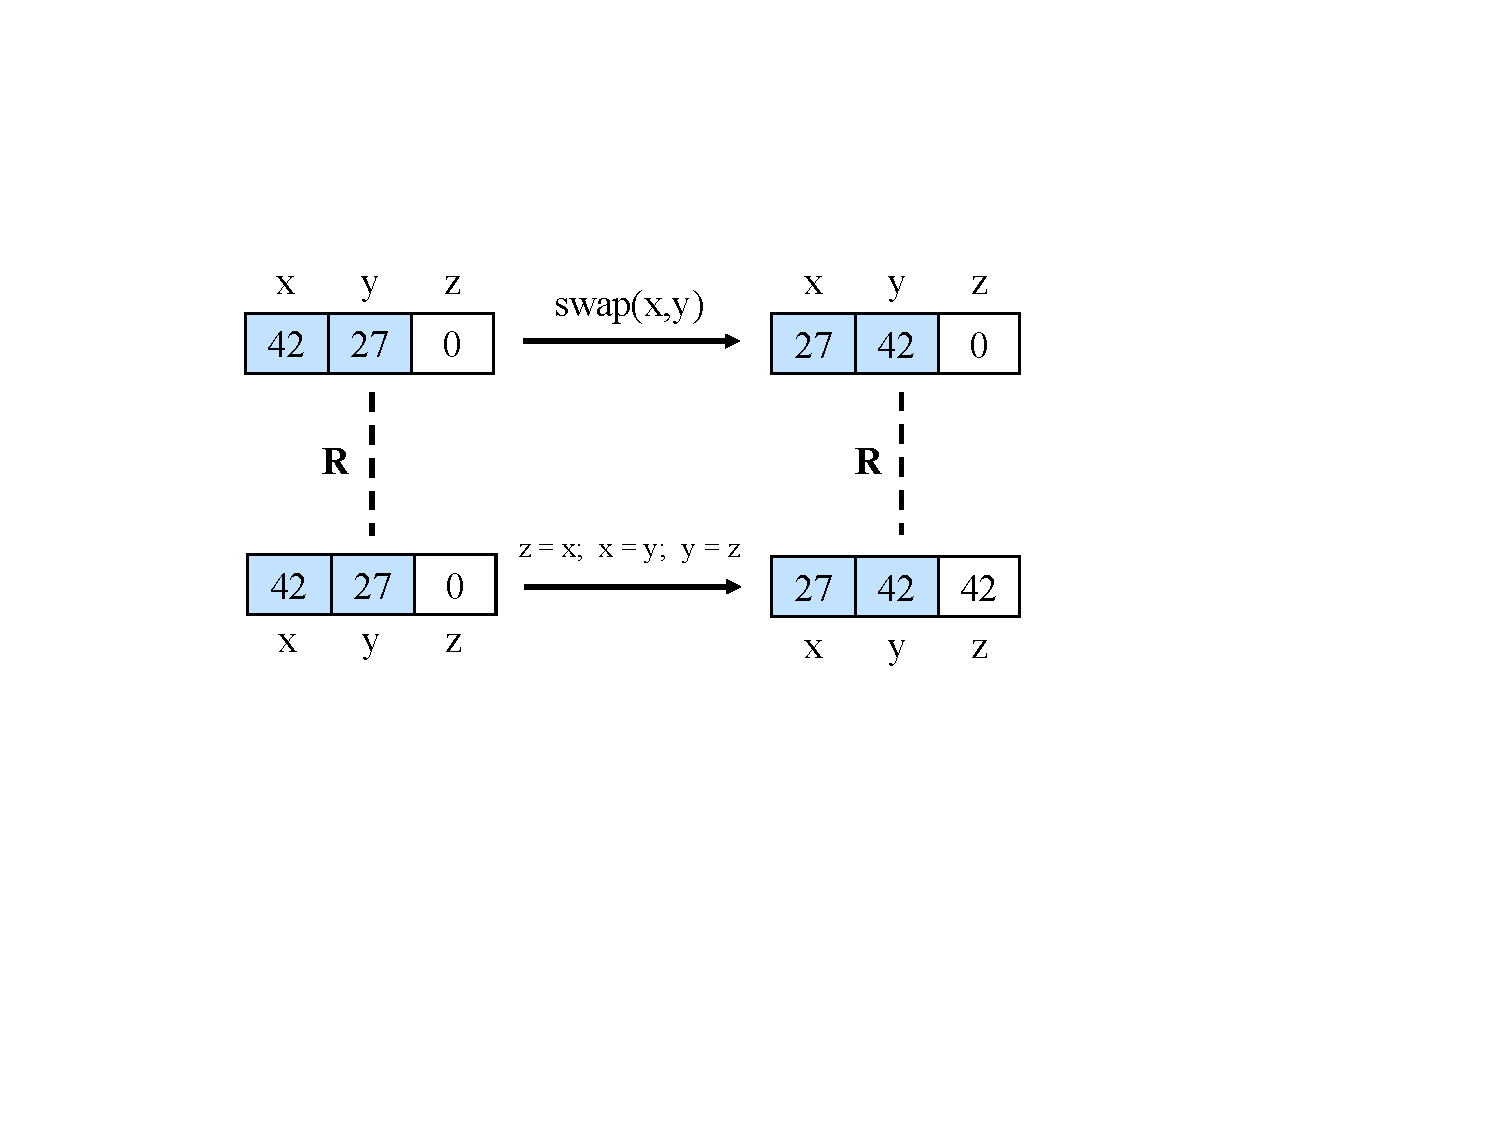
\includegraphics[scale=0.6,origin=c]{figure/paradox.pdf}}
\caption{\small{Security-Breaking Simulation: both the specification 
and implementation executions are deterministic, yet $R$ causes the 
implementation to be insecure as it relates $y$ to any value.}}
\label{paradox}
\end{figure}

When using refinement, security may not be preserved only when a 
nondeterministic program is refined into a more deterministic one. When 
using general simulations, however, even secure deterministic programs can
be simulated in an insecure way. Figure~\ref{paradox} illustrates this
point. The example assumes a program state consisting of a high-security 
(unobservable) variable $x$ and low-security (observable) variable $y$. 
The abstract action (specification) writes $0$ into $y$, while the concrete 
implementation writes $x$ into $y$. The relation $R$ relating abstract to 
concrete states simply requires that $x$ has the same value in the two 
states, and $y$ always has value $0$ in the abstract state (hence the
relation is one-to-many). It is easy to show that $R$ is a valid simulation
relation for this example (in fact, it is a valid bisimulation
relation). The abstract action is clearly secure,
as the final value of $y$ is guaranteed to be $0$ and thus has no 
dependency on the secret value of $x$. However, the implementation
is not secure: the final value of $y$ clearly depends directly
on $x$. Using the terminology above, the state observation is the value
of $y$; the abstract program always takes two indistinguishable initial 
states to indistinguishable final states, while the concrete one may not.

Our solution to this issue is obvious but fundamental. The simulation in
Figure~\ref{paradox} breaks security because security talks about 
indistinguishability of states, yet the relation $R$ fails to 
preserve indistinguishability. We therefore define a notion of
``indistinguishability-preserving simulation'', which is a normal
simulation with the additional property that two indistinguishable
states are always related to indistinguishable states. We will formalize
this in Section~\ref{methodology}, and prove that such a simulation
preserves security.

%\vspace{2mm}
\noindent
To summarize, the contributions of our work are as follows:
\begin{itemize}
\item We present a novel methodology for proving security based on
layered simulations. The security proof is done at the most
abstract layer, and can therefore express interesting policies,
including some kinds of declassification. The simulations are
specialized to preserve security, so that an
end-to-end property still holds over the most concrete layer.
No security reasoning is required over any layer besides the
abstract one.
\item We demonstrate the effectiveness of this methodology with
a major proof effort: the confidentiality between user-processes
executing over the mCertiKOS~\cite{certikos-popl} kernel.
Like mCertiKOS, our proof is fully formalized in the Coq proof 
assistant~\cite{coq}, and the code can be found in the supplementary
material~\cite{costanzo-popl16-tr}.
\end{itemize}
\end{comment}

\begin{comment}
Now that we have described our methodology for proving security,
let us revisit the initial goals:
\begin{itemize}
\item \emph{General Policies}~--- 
The observation function allows us to specify interesting security 
policies at an arbitrarily high level of abstraction. We will 
present many example policies in Section~\ref{policies}. 
\item \emph{Application to Low-Level Code}~--- 
Our solution to the refinement paradox (restricting the simulation
relation according to observations)
allows us to propagate a high-level security policy to the actual 
low-level execution.
\item \emph{Tractable Proof Effort}~--- The required proof effort is 
reasonable, as it is divided into the two
orthogonal tasks of abstracting code into a functional specification, and
then proving security over the specification. The security proof only
requires showing that single steps preserve observable equivalence;
multi-step reasoning follows automatically from induction.  
Functional specifications can be reused for proving other properties 
besides security. In Sections~\ref{casestudy-def} and~\ref{casestudy-proof}, 
we support our claim 
that the proof effort is reasonable by presenting a full security proof 
over a variant of the mCertiKOS kernel.
\item \emph{Completeness}~--- Our proof strategy achieves a satisfactory 
level of completeness, since it allows for proving an entire program secure 
even when the program manipulates data in a locally insecure way.
\end{itemize}
\end{comment}

\begin{comment}
\subsection{Security Verification of mCertiKOS}

In Sections~\ref{casestudy-def} and~\ref{casestudy-proof}, we
demonstrate our security proof methodology with a large-scale,
practical example. We prove a security property over a version of the
mCertiKOS kernel, stating that user processes are isolated from each
other. The proof is developed entirely within the Coq proof assistant,
and thus is machine-checkable.

The first step of the proof~--- abstraction of system call
implementations into functional specifications~--- was already
completed by Gu~{\em et al}~\cite{certikos-popl}. The proof presented
here deals with the second step: specifying a security policy
(observation function) and proving the security property instantiated
with this policy. While the abstraction step took about $1.5$
person-years (including the time for developing much of the refinement
framework), the security step took only $3$ person-months to complete.

To the best of our knowledge, our work is only the second
fully-formalized OS security proof to be completed; the first is the
verification effort over the seL4 
kernel~\cite{klein14,sewell11,murray12,murray13}.
There are some major shortcomings in the seL4 effort, however, that
our methodology allows us to address. One shortcoming comes from the
fact that the seL4 proof uses standard refinement rather than
contextual refinement.  This means that malicious user code (context
code) could potentially interfere with kernel state in such a way that
the refinement becomes unsound. Indeed, the seL4 security proof needs
to assume that user-level actions only touch a portion of memory state
isolated from the kernel (the user's virtual address space). In our
security verification over mCertiKOS, we \emph{prove} that users'
actions are correctly isolated to their virtual address spaces.

A second shortcoming of the seL4 proof is that it does not deal with
page faults in their model of user-level
transitions~\cite{klein14,daum14}; this is a severe limitation since
virtual memory without page fault handling would be almost unusable.
As we will show later in Section~\ref{ssec:oprim}, the security of the
page-fault handling primitive is one of the hardest and the most
tricky components in our security verification over mCertiKOS.

A third shortcoming of the seL4 proof is that their state simulation
relation is the identity relation. This means that, while they can abstract
code into atomic specifications, they cannot abstract machine state 
into more convenient forms or into purely logical state. Not only
does this make the functional specifications difficult to present
in a readable way, but it also limits the expressiveness of security 
policies. Note that they completely elide the refinement
paradox issue by never abstracting program state.

A fourth issue with the seL4 proof is that refinement is only verified
for implementations written in C. Anything written directly in
assembly is assumed to have been implemented and abstracted correctly.
This is particularly relevant for an operating system, since there is
some functionality such as context switching that \emph{must} be
implemented in assembly. Our contextual refinement framework, on the
other hand, guarantees that the functional specification is a correct
abstraction of the actual implementation, regardless of whether the
implementation is written in C or assembly. Thus we can be certain
that our security theorem propagates down to the actual
implementation, even across assembly primitives like context switch.
\end{comment}

}
